\vspace{12pt}
\section{Effect of Gaseous Environment on Conductivity of Bulk Samples}

\begin{figure}
\centering
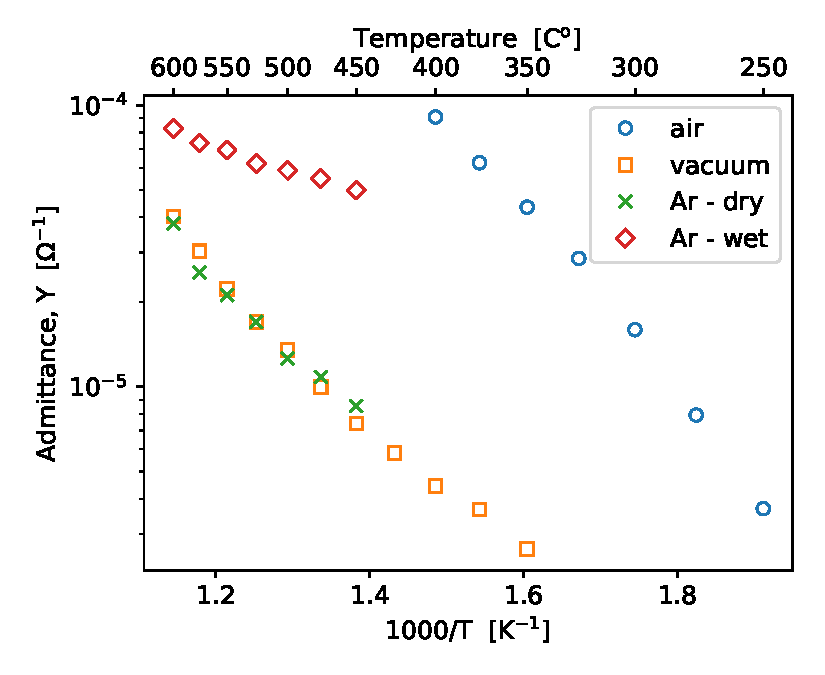
\includegraphics{Figures/bzgxs10-gas-env-comparison-2.pdf}
  \caption{Difference in conductivity measurements showing the dependence on gaseous environment on conduction. Sample is a pellet of Gd:BaZrO$_3$ made by solid state reaction method.}
  \label{target:fig:gas_comp}
\end{figure}

Conductivity measurements in various gaseous environments offer important indications about the dominant conduction mechanisms in a sample. It is generally understood that electrical transport in doped barium zirconate is dominated by oxide ions under inert gas environment. This is because the large concentration of oxygen vacancies in the system readily provides sites that effectively mediate oxide-ion diffusion. On the other hand, the presence of an atmosphere that leads to the ``filling'' of oxygen vacancies will suppress oxygen-ion conduction. This is expected to be the case when samples are immersed in an hydroxyl-rich gaseous environment. Suppression of oxygen-ion conduction may enable the observation of protonic conduction if sufficient H$^+$ ions are available. A final process is also possible in highly oxidizing environments where oxidation of a vacancy can lead to the introduction of electron holes according to the reaction \cite{Yamazaki2008}:
\begin{equation}
    \mathrm{\frac{1}{2}O_2(gas) + V_O^{\bullet\bullet}  \leftrightarrow O_O^x + 2 h^{\bullet}}
    \label{eq:bulk:holeConduction}
\end{equation}
Finally, environments that promote the ``filling'' of  oxygen vacancies (by e.g., O$_2$ ions themselves) without the presence protonic species, may suppress both, protonic and oxide-ion conduction, revealing any other non-ionic conduction mechanisms. In order to evaluate the presence of these various mechanisms in our samples, we have conducted conductivity measurements of pellets under vacuum, exposed to dry Ar, Ar saturated in water vapor, ambient air, and forming gas (5\% H$_2$ in balance of N$_2$) saturated with water vapor.  The effects of some of these gaseous environments can be seen in Figure \ref{target:fig:gas_comp}. As seen in the figure, measurements under ambient air lead to the highest values of conductivity in the 400-600\textdegree C temperature range. These high conductivities are likely to be associated with electronic or hole conduction in the samples. On the other hand, measurements under dry conditions with no availability of oxygen species (vacuum or Ar-dry), reveal substantially lower conductivity values with a temperature behavior characteristic of a much higher activation energy. These lower values are most likely due to transport dominated by oxide-ion conduction. Interestingly, when a saturation concentration of OH$^-$ is made available (Ar-wet), a substantial change in conduction is observed, which is possibly indicative of the activation of proton conduction. 

